\section{Wyniki}
\label{sec:wyniki}

W niniejszej sekcji prezentujemy wyniki sześciu eksperymentów odpowiadających
hipotezom H1--H6, wszystkie przeprowadzone na klasycznej planszy 8$\times$8.
Wszystkie odsetki wygranych raportowane są wraz z 95\%
przedziałami ufności wyliczanymi metodą Wilsona \cite{wilson1927probable}.

\subsection{H1: RAVE vs vanilla UCT}
\label{sec:wyniki-h1}

\begin{figure}[ht]
    \centering
    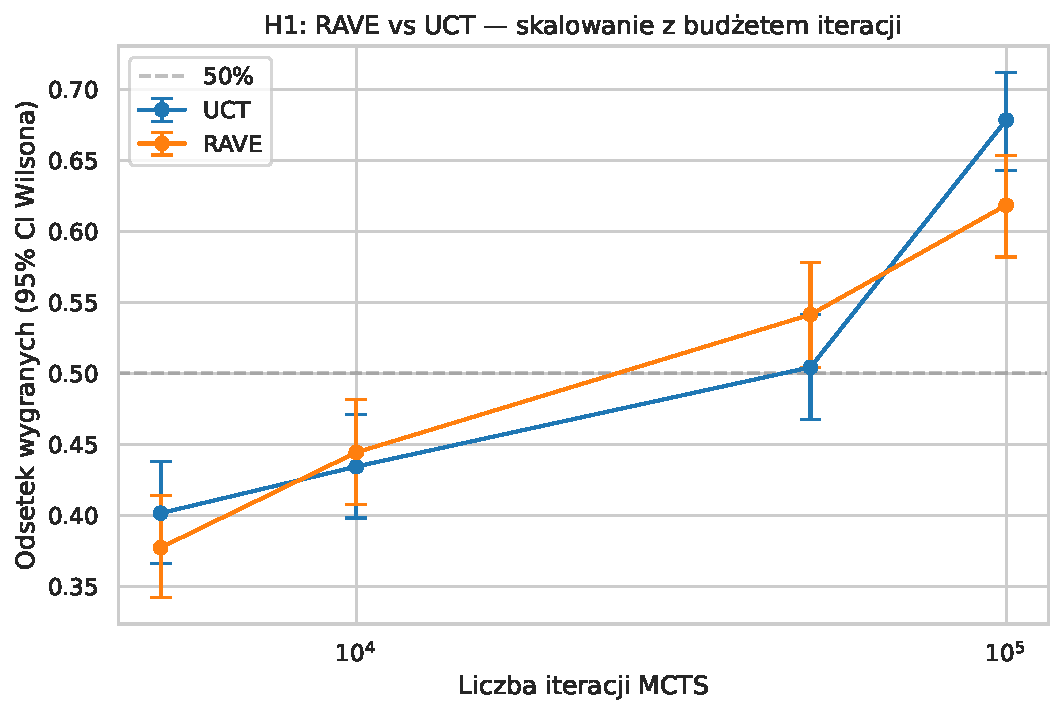
\includegraphics[width=0.85\textwidth]{figures/h1_rave_vs_uct}
    \caption{Skalowanie odsetków wygranych RAVE i UCT z budżetem iteracji
    (8$\times$8, turniej round-robin). Punkty pokazują ogólny win-rate każdego
    agenta we wszystkich rozegranych przez niego partiach, słupki błędów to
    95\% CI Wilsona. Linia 50\% oznacza neutralność. Obie metody zyskują z budżetem;
    RAVE nie wyprzedza UCT przy żadnym budżecie.}
    \label{fig:h1}
\end{figure}

\paragraph{Dane liczbowe --- bezpośrednie mecze RAVE vs UCT przy tym samym
budżecie (n=100 partii na budżet):}
\begin{center}
\begin{tabular}{rcccc}
\toprule
\textbf{Budżet} & \textbf{RAVE wygrywa} & \textbf{Win-rate} & \textbf{$p$ (vs 0,5)} & \textbf{Status} \\
\midrule
5\,000   & 49/100 & 49,0\% & 0,92 & parytet \\
10\,000  & 48/100 & 48,0\% & 0,76 & parytet \\
50\,000  & 54/100 & 54,0\% & 0,48 & parytet \\
100\,000 & 39/100 & \textbf{39,0\%} & 0,035 & RAVE gorszy \\
\bottomrule
\end{tabular}
\end{center}

Hipoteza H1 jest \emph{sfalsyfikowana}: RAVE nie wygrywa istotnie z vanilla UCT
przy żadnym budżecie, a przy 100\,000 iteracji \emph{przegrywa} istotnie
statystycznie (39,0\%, $p = 0{,}035$). Rezultat jest odmienny od oczekiwań
literaturowych z dziedziny Go, gdzie RAVE przewyższa vanilla UCT przy każdym
praktycznym budżecie \cite{gelly2011monte}.

Interpretujemy to następująco: RAVE akumuluje wartości AMAF przez wszystkie
pozycje w drzewie i symulacjach, zakładając przesuwalność wartości ruchu
(translation invariance). Założenie to zachodzi w Go (kamień postawiony
w punkcie $X$ ma podobną wartość w różnych kontekstach), ale załamuje się
w Breakthrough, gdzie wartość ruchu (np.\ ,,pionek z pola $X$ na $Y$'') silnie
zależy od reszty pozycji. Sygnał AMAF jest więc niemal nieinformatywny;
przy największym budżecie staje się wręcz szkodliwy, podczas gdy vanilla UCT
efektywnie wykorzystuje rosnący budżet do precyzowania szacunków per-stan.
Zauważmy, że poprawność samej implementacji RAVE potwierdziliśmy niezależnie
(sekcja~\ref{sec:llm}): przy zneutralizowanym członie AMAF ($\beta \to 0$)
RAVE odtwarza siłę UCT, co dowodzi, że obserwowany spadek pochodzi z heurystyki
AMAF, a nie z błędu w szkielecie algorytmu.

\subsection{H2: Progressive Bias vs vanilla UCT}
\label{sec:wyniki-h2}

\begin{figure}[ht]
    \centering
    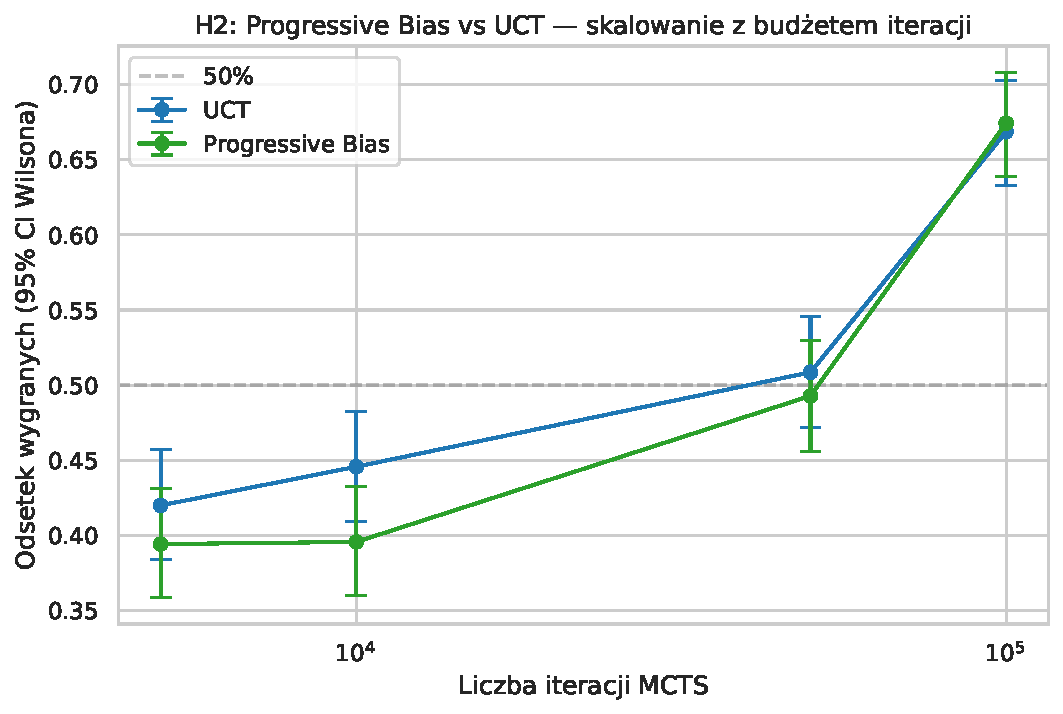
\includegraphics[width=0.85\textwidth]{figures/h2_pb_vs_uct}
    \caption{Skalowanie odsetków wygranych Progressive Bias i UCT (8$\times$8).
    Człon bias w selekcji oparty na heurystyce porządkowania ruchów ($\pi/1000$).
    Krzywe PB i UCT pokrywają się na całym zakresie budżetów --- brak
    statystycznie istotnej różnicy.}
    \label{fig:h2}
\end{figure}

\paragraph{Dane liczbowe --- bezpośrednie mecze PB vs UCT przy tym samym
budżecie (n=100 partii na budżet):}
\begin{center}
\begin{tabular}{rcccc}
\toprule
\textbf{Budżet} & \textbf{PB wygrywa} & \textbf{Win-rate} & \textbf{$p$ (vs 0,5)} & \textbf{Status} \\
\midrule
5\,000   & 50/100 & 50,0\% & 1,00 & parytet \\
10\,000  & 43/100 & 43,0\% & 0,19 & parytet \\
50\,000  & 55/100 & 55,0\% & 0,37 & parytet \\
100\,000 & 46/100 & 46,0\% & 0,48 & parytet \\
\bottomrule
\end{tabular}
\end{center}

W żadnym z testowanych budżetów PB nie pokonuje UCT istotnie statystycznie ---
wszystkie wyniki oscylują wokół 50\% ($p > 0{,}19$). Hipoteza H2 jest zatem
\emph{niejednoznaczna}: nie można odrzucić hipotezy zerowej o braku różnicy
względem UCT.

Interpretacja: heurystyka użyta w członie bias to znormalizowana funkcja
porządkowania ruchów (Algorytm~2) --- prostsza niż pełna funkcja ewaluacji
w agentcie heurystycznym (sekcja~\ref{sec:wyniki-h3}). Wiedza domenowa
wstrzykiwana przez PB jest więc ograniczona, a jej wpływ dodatkowo zanika
wraz z liczbą odwiedzin węzła ($H/(n+1)$). W efekcie PB zachowuje dobrą
zbieżność asymptotyczną UCT, lecz nie daje mierzalnej przewagi w tej grze.

\subsection{H3: Heurystyka alpha-beta vs UCT --- poszukiwanie cross-over}
\label{sec:wyniki-h3}

\begin{figure}[ht]
    \centering
    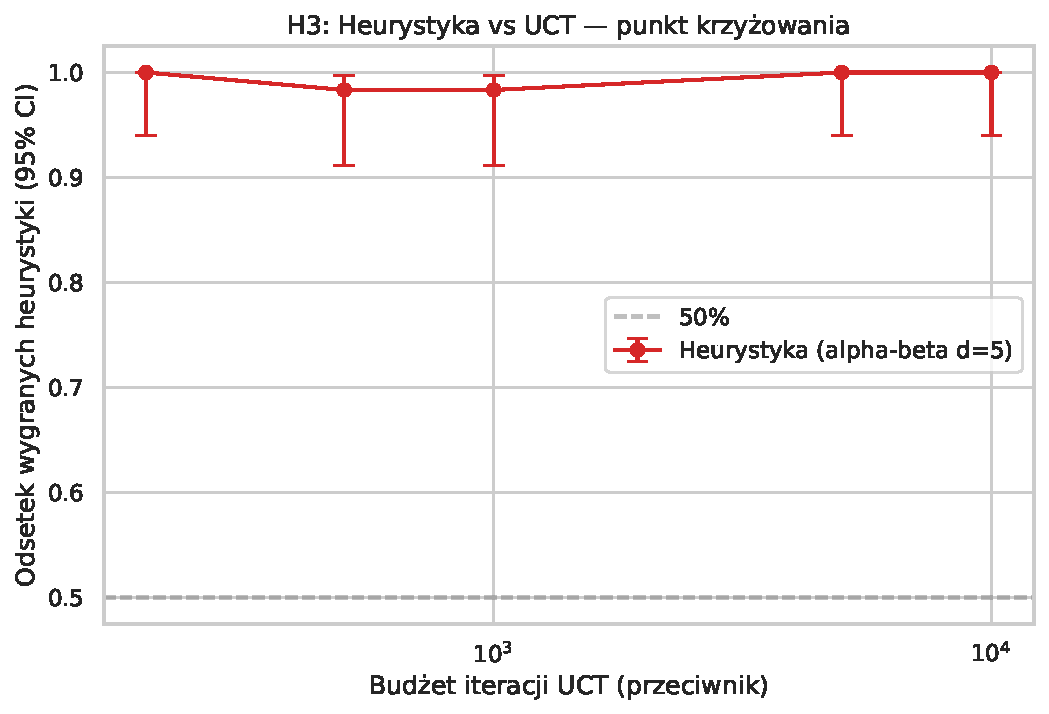
\includegraphics[width=0.85\textwidth]{figures/h3_heuristic_vs_uct}
    \caption{Odsetek wygranych heurystyki (alpha-beta z głębokością 5) względem
    rosnącego budżetu iteracji UCT na planszy 8$\times$8. Oś X logarytmiczna.
    Heurystyka miażdży UCT w całym testowanym zakresie; przy 100\,000 iteracji
    nadal wygrywa 94\% partii --- punkt krzyżowania nie zostaje osiągnięty.}
    \label{fig:h3}
\end{figure}

\paragraph{Dane liczbowe (n=100 partii na budżet, bezpośrednie mecze
heurystyka vs UCT):}

\begin{center}
\begin{tabular}{rcccc}
\toprule
\textbf{Budżet UCT} & \textbf{Heur wygrywa} & \textbf{Win-rate} & \textbf{95\% CI} & \textbf{UCT czas/ruch} \\
\midrule
500      & 99/100  & 99,0\%  & [94,6; 99,8] & $\sim$0,005 s \\
1\,000   & 100/100 & 100,0\% & [96,3; 100]  & $\sim$0,01 s \\
5\,000   & 98/100  & 98,0\%  & [93,0; 99,4] & $\sim$0,05 s \\
10\,000  & 98/100  & 98,0\%  & [93,0; 99,4] & $\sim$0,10 s \\
50\,000  & 94/100  & 94,0\%  & [87,5; 97,2] & $\sim$0,50 s \\
100\,000 & 94/100  & 94,0\%  & [87,5; 97,2] & $\sim$0,97 s \\
\bottomrule
\end{tabular}
\end{center}

Heurystyka pozostaje dominująca w całym praktycznym zakresie. Pierwsza część
hipotezy (wyższość heurystyki przy niskich budżetach) jest spektakularnie
potwierdzona. Druga część (cross-over przy wysokich budżetach) jest
\emph{nieosiągnięta}: win-rate maleje bardzo łagodnie (z 99\% przy UCT(500)
do 94\% przy UCT(100\,000)), pozostając daleko od parytetu. Ekstrapolując ten
trend, teoretyczny cross-over (50\%) leży znacznie powyżej $10^6$ iteracji ---
daleko poza praktycznym zakresem (UCT(100\,000) zajmuje już $\sim$1\,s/ruch).
Na większej planszy 8$\times$8 (głębsze, bardziej taktyczne partie) przewaga
heurystyki jest nawet wyraźniejsza niż przy mniejszych wariantach, ponieważ
losowe symulacje słabiej przybliżają wartość pozycji.

Wynik jest mocnym argumentem za stosowaniem prostych deterministycznych
graczy z funkcją ewaluacji w grach o wyraźnej strukturze taktycznej
i umiarkowanym branching factor. Heurystyka w naszej implementacji wybiera
ruch w $\sim$10 ms (depth 5, 8$\times$8), więc partia $\sim$60 ruchów to
poniżej sekundy --- rzędy wielkości taniej niż UCT(100\,000), a przy tym
istotnie silniej grające.

\subsection{H4: Przewaga pierwszego gracza}
\label{sec:wyniki-h4}

\begin{figure}[ht]
    \centering
    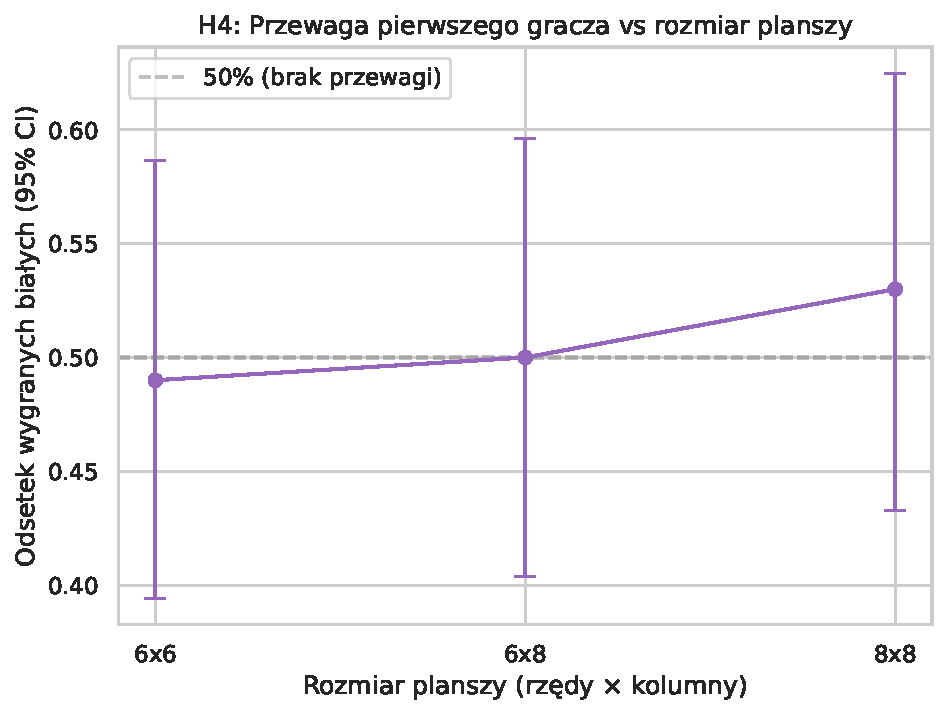
\includegraphics[width=0.5\textwidth]{figures/h4_first_player_advantage}
    \caption{Odsetek wygranych białych (pierwszego gracza) w symetrycznym
    turnieju UCT(5000) vs UCT(5000) na planszy 8$\times$8. Linia 50\% oznacza
    brak przewagi; 95\% CI Wilsona zawiera 50\%.}
    \label{fig:h4}
\end{figure}

\paragraph{Dane liczbowe (n=500 partii):}
Białe wygrały 247/500 = \textbf{49,4\%} partii, 95\% CI Wilsona $[45{,}0\%;\ 53{,}8\%]$
(średnia długość partii ok. 59 ruchów). Przedział obejmuje 50\%, brak więc
istotnej statystycznie przewagi pierwszego gracza.

Hipoteza H4 jest sfalsyfikowana: nie stwierdzamy istotnej statystycznie przewagi
białych. Szerokość CI (ok. $\pm$4,4 pp) jest wystarczająco wąska, by uznać,
że ewentualna ,,prawdziwa'' przewaga jest mniejsza niż 4 pp --- co metodologicznie
odpowiada brakowi przewagi praktycznej.

Interpretacja:
\begin{itemize}[nosep]
    \item Przy MCTS o zbliżonej sile oboje gracze grają sub-optymalnie
          w sposób przybliżonie symetryczny --- przewaga tempa pierwszego
          ruchu zostaje ,,wyzerowana'' przez błędy obu stron.
    \item Możliwe, że przy perfekcyjnej grze (jak w rozwiązanych wariantach
          6$\times$5 \cite{saffidine2011solving} i 6$\times$6
          \cite{bjornsson2026solving}, gdzie wygrywa pierwszy gracz) białe
          rzeczywiście mają przewagę, lecz UCT z 5000 iteracji nie zbliża się
          do tej granicy.
\end{itemize}

\subsection{H5: Strojenie stałej eksploracji $c$}
\label{sec:wyniki-h5}

\begin{figure}[ht]
    \centering
    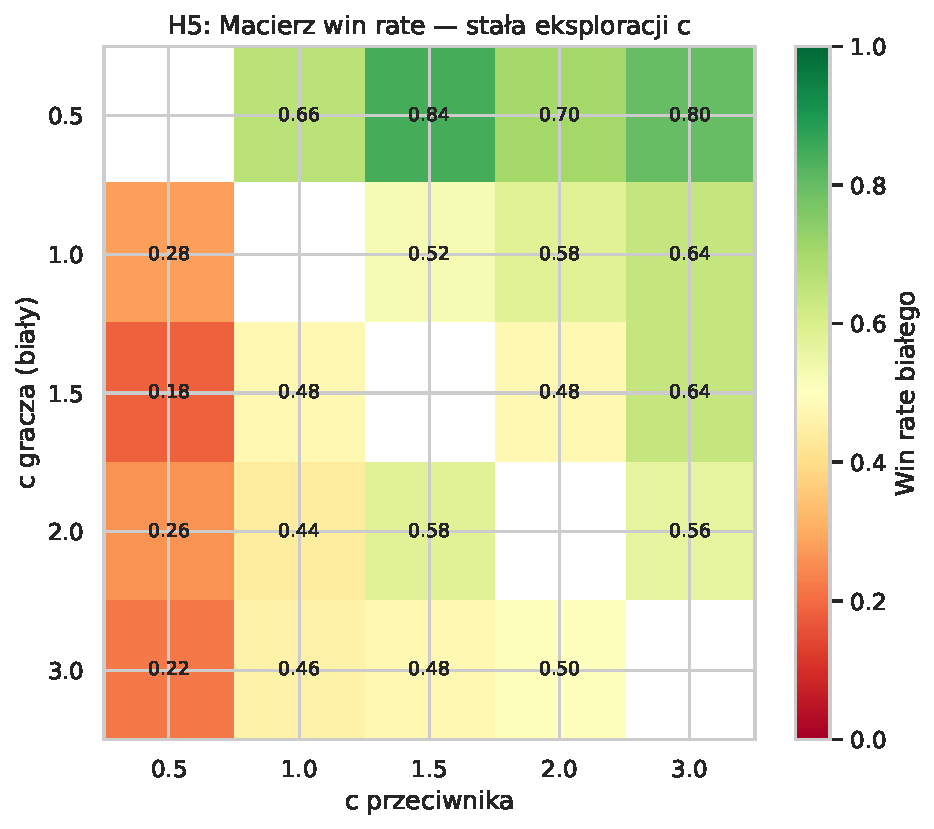
\includegraphics[width=0.7\textwidth]{figures/h5_c_heatmap}
    \caption{Macierz win-rate białych dla turnieju round-robin pięciu wartości
    stałej eksploracji $c$ (UCT 10\,000 iteracji, 8$\times$8). Wiersz --- $c$ gracza
    białego, kolumna --- $c$ przeciwnika. Im niższe $c$ wiersza, tym wyraźniej
    zielony (więcej wygranych): $c = 0{,}5$ dominuje całą tabelę.}
    \label{fig:h5_heatmap}
\end{figure}

\begin{figure}[ht]
    \centering
    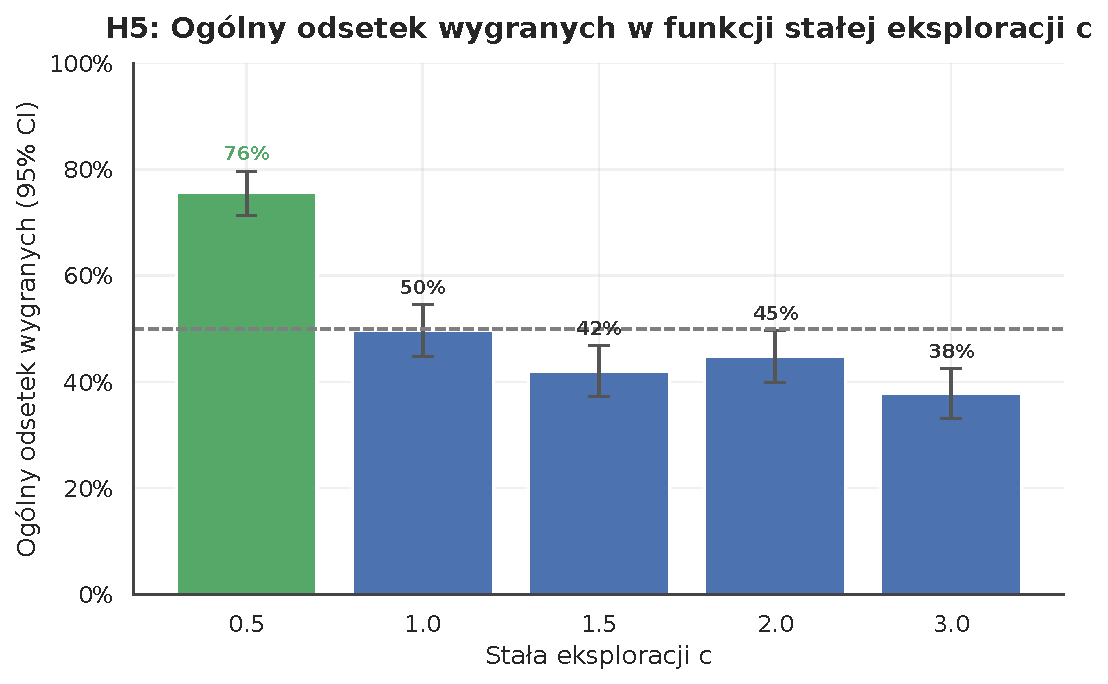
\includegraphics[width=0.7\textwidth]{figures/h5_c_bar}
    \caption{Ogólny win-rate każdej wartości $c$ (uśredniony po obu kolorach
    i wszystkich przeciwnikach). Trend jest w przybliżeniu monotonicznie malejący;
    brak wewnętrznego maksimum w badanym zakresie.}
    \label{fig:h5_bar}
\end{figure}

\paragraph{Dane liczbowe (n=400 partii na wartość $c$):}
\begin{center}
\begin{tabular}{rcccc}
\toprule
\textbf{$c$} & \textbf{Win-rate} & \textbf{95\% CI} & \textbf{$p$ (vs 0,5)} & \textbf{Status} \\
\midrule
0,5 & \textbf{75,7\%} & [71,3; 79,7] & $<10^{-4}$ & najlepsza \\
1,0 & 49,7\% & [44,9; 54,6] & 0,96 & neutralna \\
1,5 & 42,0\% & [37,3; 46,9] & 0,0016 & poniżej 50\% \\
2,0 & 44,8\% & [40,0; 49,6] & 0,040 & poniżej 50\% \\
3,0 & 37,8\% & [33,1; 42,6] & $<10^{-4}$ & najgorsza \\
\bottomrule
\end{tabular}
\end{center}

Hipoteza H5 (istnienie wewnętrznego optimum $c^\star$ o kształcie odwróconego U)
\emph{nie znajduje potwierdzenia} w badanym zakresie. Najsilniejsza okazuje się
\emph{najniższa} testowana wartość $c = 0{,}5$ (75,7\% wygranych, wysoce istotnie),
a win-rate maleje wraz ze wzrostem $c$ --- nie obserwujemy spadku przy małym $c$,
który zamykałby krzywą w kształt odwróconego U. Co więcej, teoretyczna wartość
$c = \sqrt{2} \approx 1{,}41$ (okolice $c = 1{,}5$) wypada wyraźnie poniżej parytetu.

Interpretacja: Breakthrough jest grą silnie taktyczną, w której kluczowe są
konkretne, wymuszone warianty, a nie szerokie zwiedzanie drzewa. Niski $c$
(nacisk na eksploatację) pozwala MCTS głębiej drążyć obiecujące linie, co
przekłada się na realną przewagę. Optymalne $c^\star$ leży zatem \emph{na lub
poniżej} dolnej granicy testowanego zakresu --- co stanowi praktyczną wskazówkę
do strojenia UCT w tej grze i sugeruje rozszerzenie eksperymentu o $c \in \{0{,}1,\ 0{,}25\}$.

\subsection{H6: Czas decyzji w funkcji numeru ruchu}
\label{sec:wyniki-h6}

\begin{figure}[ht]
    \centering
    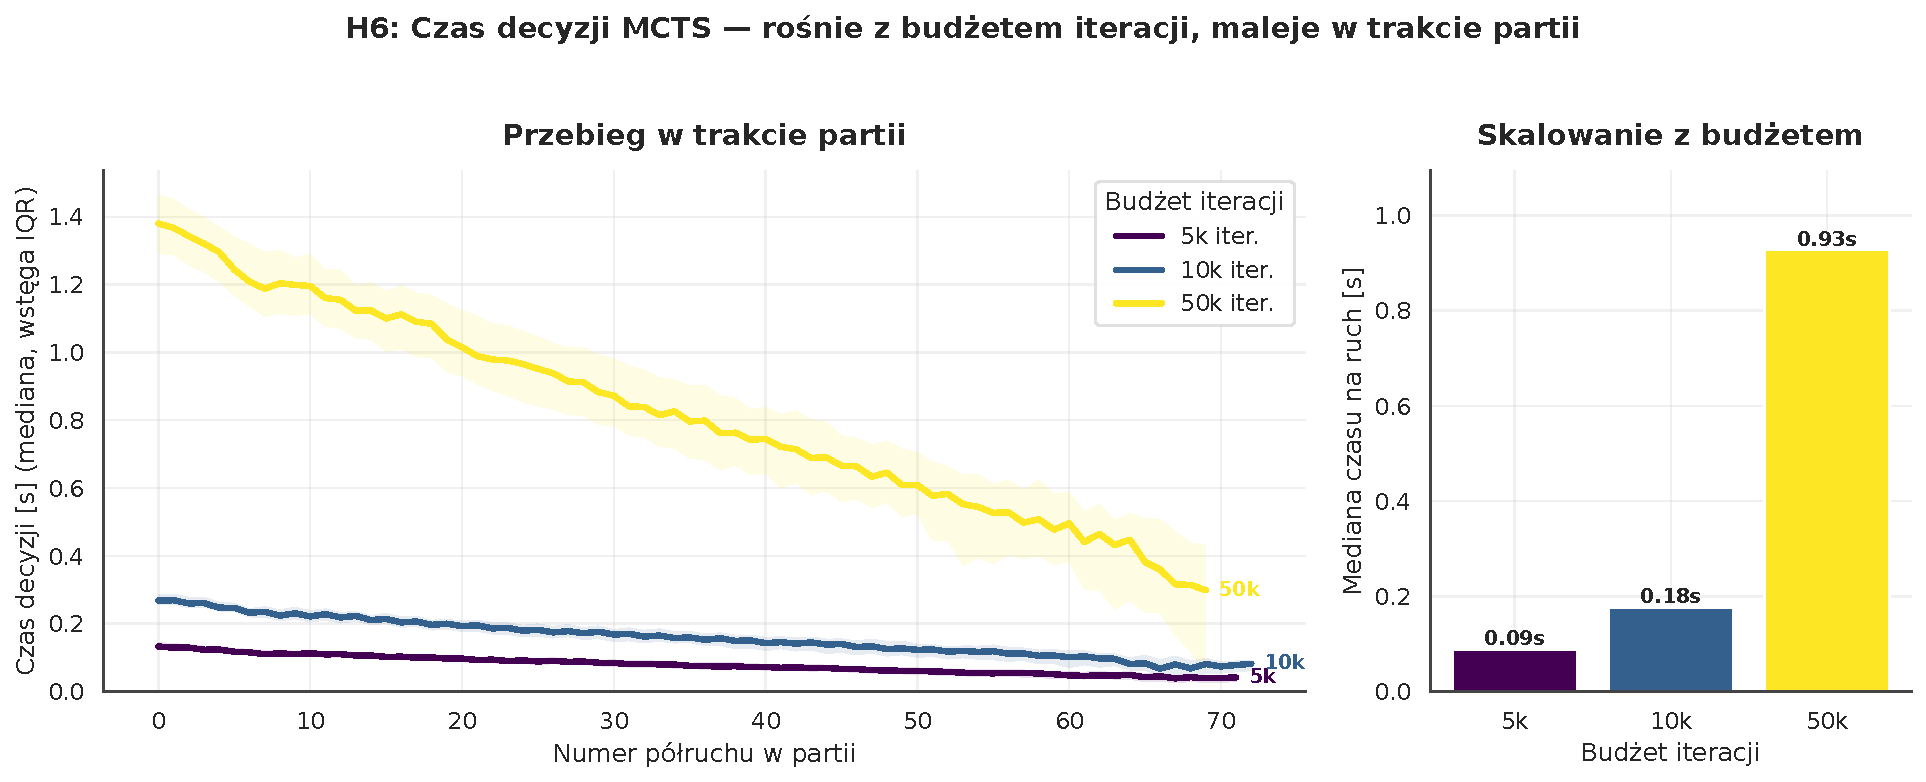
\includegraphics[width=0.95\textwidth]{figures/h6_decision_time}
    \caption{Średni czas decyzji UCT w funkcji numeru ruchu, w rozbiciu na budżet
    iteracji (8$\times$8). Czas jest najwyższy w otwarciu i maleje monotonicznie
    w trakcie partii. Charakterystyczny ząbkowany kształt wynika z naprzemiennej
    gry agentów o różnych budżetach (kolejne ruchy wykonują różni gracze).}
    \label{fig:h6}
\end{figure}

\paragraph{Średni czas decyzji wg budżetu iteracji:}
\begin{center}
\begin{tabular}{rcc}
\toprule
\textbf{Budżet UCT} & \textbf{Średni czas/ruch} & \textbf{Odch.\ std.} \\
\midrule
5\,000   & 0,298 s & 0,364 s \\
10\,000  & 0,354 s & 0,389 s \\
50\,000  & 0,517 s & 0,453 s \\
\bottomrule
\end{tabular}
\end{center}

Hipoteza H6 (czas decyzji rośnie w środkowej fazie gry) jest \emph{sfalsyfikowana}.
Wbrew oczekiwaniom, średni czas na ruch jest \emph{najwyższy w otwarciu}
i maleje monotonicznie w miarę postępu partii --- nie obserwujemy maksimum
w ruchach 15--40. Wyjaśnienie tkwi w naturze kosztu pojedynczej iteracji MCTS:
przy stałym budżecie iteracji dominującym kosztem jest długość losowej symulacji
(rolloutu do stanu terminalnego), a ta jest najdłuższa na początku gry i kurczy
się wraz ze zbliżaniem do końcówki. Większy branching factor w środkowej fazie
\emph{nie} podnosi kosztu ruchu, ponieważ liczba iteracji jest ustalona.
Zgodnie z oczekiwaniem skaluje się natomiast czas z budżetem (0,30 s $\to$
0,52 s dla 5k $\to$ 50k iteracji).

\subsection{Synteza ilościowa}

Tabela~\ref{tab:synteza} podsumowuje status każdej hipotezy.

\begin{table}[ht]
\centering
\caption{Synteza wyników eksperymentalnych.}
\label{tab:synteza}
\begin{tabular}{p{3cm}p{6cm}p{4cm}}
\toprule
\textbf{Hipoteza} & \textbf{Wynik} & \textbf{Status} \\
\midrule
H1: RAVE > UCT &
49,0 / 48,0 / 54,0 / 39,0\%
(@ 5k / 10k / 50k / 100k iter) &
Sfalsyfikowana \\
\midrule
H2: PB > UCT &
50,0 / 43,0 / 55,0 / 46,0\%
(@ 5k / 10k / 50k / 100k iter) &
Niejednoznaczna \\
\midrule
H3: heurystyka > UCT przy niskim budżecie, < UCT przy wysokim &
99\% $\to$ 94\%
(@ 500--100\,000 iter) &
Częściowo potwierdzona \\
\midrule
H4: białe mają przewagę &
49,4\% wygranych białych
(8$\times$8, n=500) &
Sfalsyfikowana \\
\midrule
H5: $c$ ma nieliniowy wpływ (optimum $c^\star$) &
najlepsze $c=0{,}5$ (75,7\%), monotoniczny spadek do $c=3{,}0$ (37,8\%) &
Sfalsyfikowana \\
\midrule
H6: czas decyzji rośnie w środku gry &
czas maleje monotonicznie od otwarcia &
Sfalsyfikowana \\
\bottomrule
\end{tabular}
\end{table}
